\subsection{Dataset}
\label{sec:dataset}

\begin{figure*}[htbp]
\centering
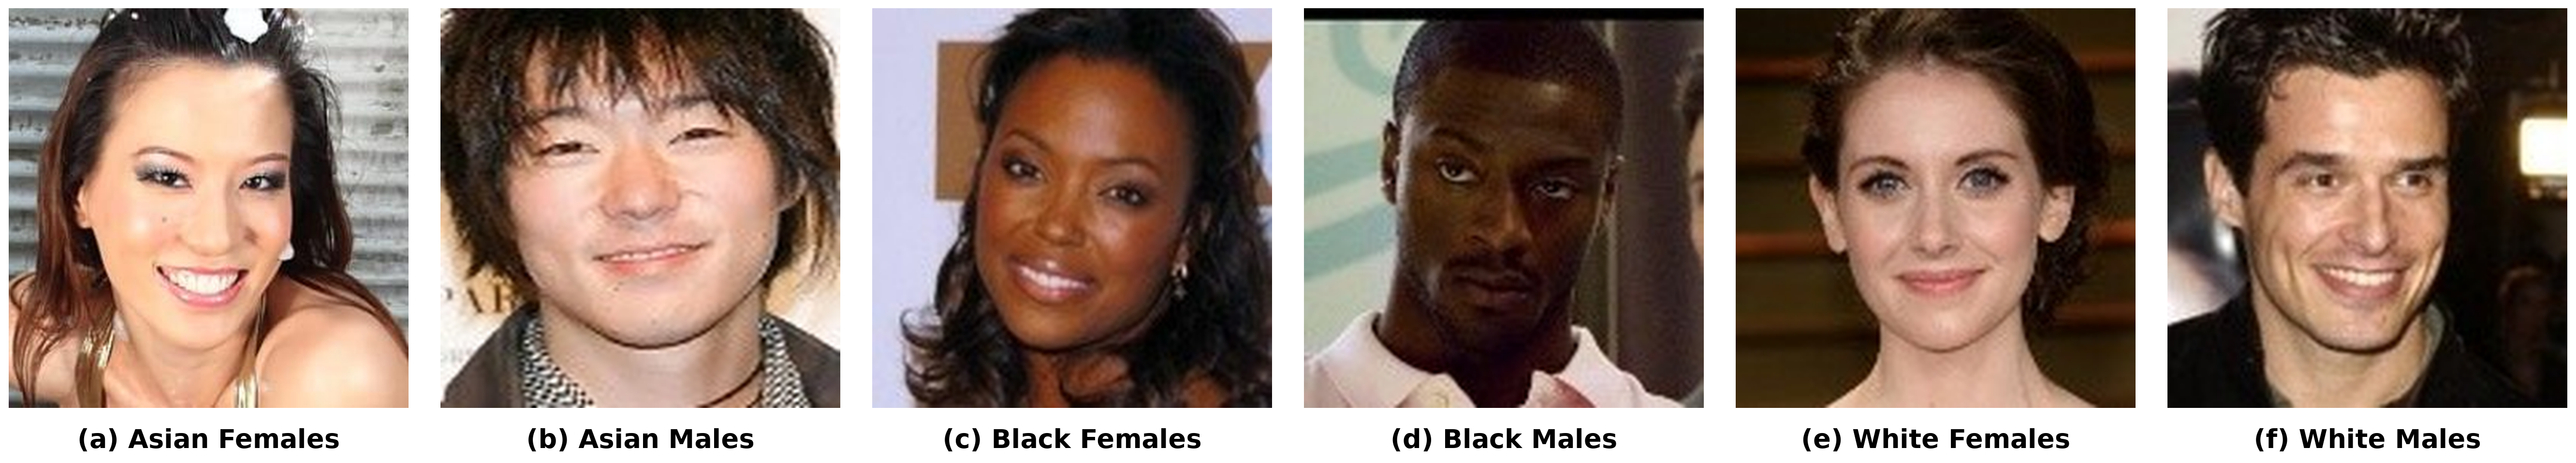
\includegraphics[width=\textwidth]{sample_demogpairs_v2.png}
\caption{Sample Images of the DemogPairs Dataset across Six Intersectional Demographic Subgroups: (a) Asian Females, (b) Asian Males, (c) Black Females, (d) Black Males, (e) White Females, and (f) White Males.}
\label{fig:2}
\end{figure*}

Eksperimen dalam penelitian ini memanfaatkan dataset DemogPairs yang dikembangkan oleh Hupont dan Fernández~\cite{ref25}. Dataset ini dirancang secara khusus sebagai tolok ukur pengujian biometrik verifikasi wajah untuk mengevaluasi dampak ketimpangan demografis pada sistem pengenalan wajah mendalam. Korpus ini memuat total 10.800 citra wajah yang terdistribusi secara seimbang sempurna ke dalam enam subkelompok demografis interseksional, yaitu persilangan antara tiga kelompok ras makro (Asian, Black, dan White) serta dua kategori gender biner (Female dan Male). Struktur dataset mencakup 600 subjek atau identitas unik, dengan alokasi seragam tepat 100 individu untuk setiap subkelompok demografis. Setiap identitas diwakili oleh tepat 18 citra wajah terkontrol yang mencakup variasi pose kepala, ragam ekspresi afektif, dan kondisi pencahayaan terstandar, sehingga menghasilkan 1.800 citra per subkelompok. Distribusi kelas yang seimbang ini menciptakan lingkungan evaluasi yang terkontrol untuk menganalisis disparitas performa klasifikasi antarsubkelompok secara objektif tanpa terdistorsi oleh ketidakseimbangan jumlah sampel. Contoh citra wajah dari keenam subkelompok demografis tersebut disajikan pada Figure~\ref{fig:2}.

Untuk menjamin integritas evaluasi dan mengeliminasi risiko kebocoran identitas secara mutlak (0\% kebocoran), penelitian ini menerapkan protokol Strict Subject-Disjoint Partitioning. Sebanyak 600 identitas unik dipisahkan secara deterministik menjadi 480 subjek untuk set latih (80\%) dan 120 subjek untuk set uji held-out (20\%). Pembagian ini dilakukan secara terstratifikasi ketat pada keenam subkelompok demografis, sehingga menghasilkan alokasi seimbang berupa 80 subjek latih (1.440 citra) dan 20 subjek uji (360 citra) per subkelompok. Skema partisi ini menghasilkan total 8.640 citra pada set latih dan 2.160 citra pada set uji held-out, sebagaimana dirinci pada Table~\ref{tab:1}. Seluruh subjek uji bersifat independen dan belum pernah dilihat oleh model selama proses pelatihan maupun penalaan hyperparameter. Pada tahapan prapemrosesan data, setiap citra wajah berformat terpusat dikonversi ke format 3-channel Red, Green, Blue (RGB) dan diubah resolusinya menjadi 224 $\times$ 224 piksel. Intensitas piksel dinormalisasi secara channel-wise mengikuti parameter rata-rata dan deviasi standar yang sesuai dengan konfigurasi pra-latih masing-masing checkpoint vision transformer. Tidak ada augmentasi buatan sintetis yang diterapkan dalam alur kerja ini demi menguji kapasitas generalisasi representasi fitur secara murni.

\begin{table*}[htbp]
\caption{DemogPairs Dataset Partition and Subject-Disjoint Demographic Subgroup Distribution.}
\label{tab:1}
\label{tab:I}
\centering
\begin{tabular}{lcccccc}
\toprule
Subkelompok Demografis & Subjek Latih & Citra Latih & Subjek Uji (Held-Out) & Citra Uji (Held-Out) & Total Subjek & Total Citra \\
\midrule
Asian Females & 80 & 1.440 & 20 & 360 & 100 & 1.800 \\
Asian Males & 80 & 1.440 & 20 & 360 & 100 & 1.800 \\
Black Females & 80 & 1.440 & 20 & 360 & 100 & 1.800 \\
Black Males & 80 & 1.440 & 20 & 360 & 100 & 1.800 \\
White Females & 80 & 1.440 & 20 & 360 & 100 & 1.800 \\
White Males & 80 & 1.440 & 20 & 360 & 100 & 1.800 \\
\midrule
\textbf{Total} & \textbf{480} & \textbf{8.640} & \textbf{120} & \textbf{2.160} & \textbf{600} & \textbf{10.800} \\
\bottomrule
\end{tabular}
\end{table*}
